\chapter{System Design and Implementation}

\begin{figure}[htbp]
    \centering
    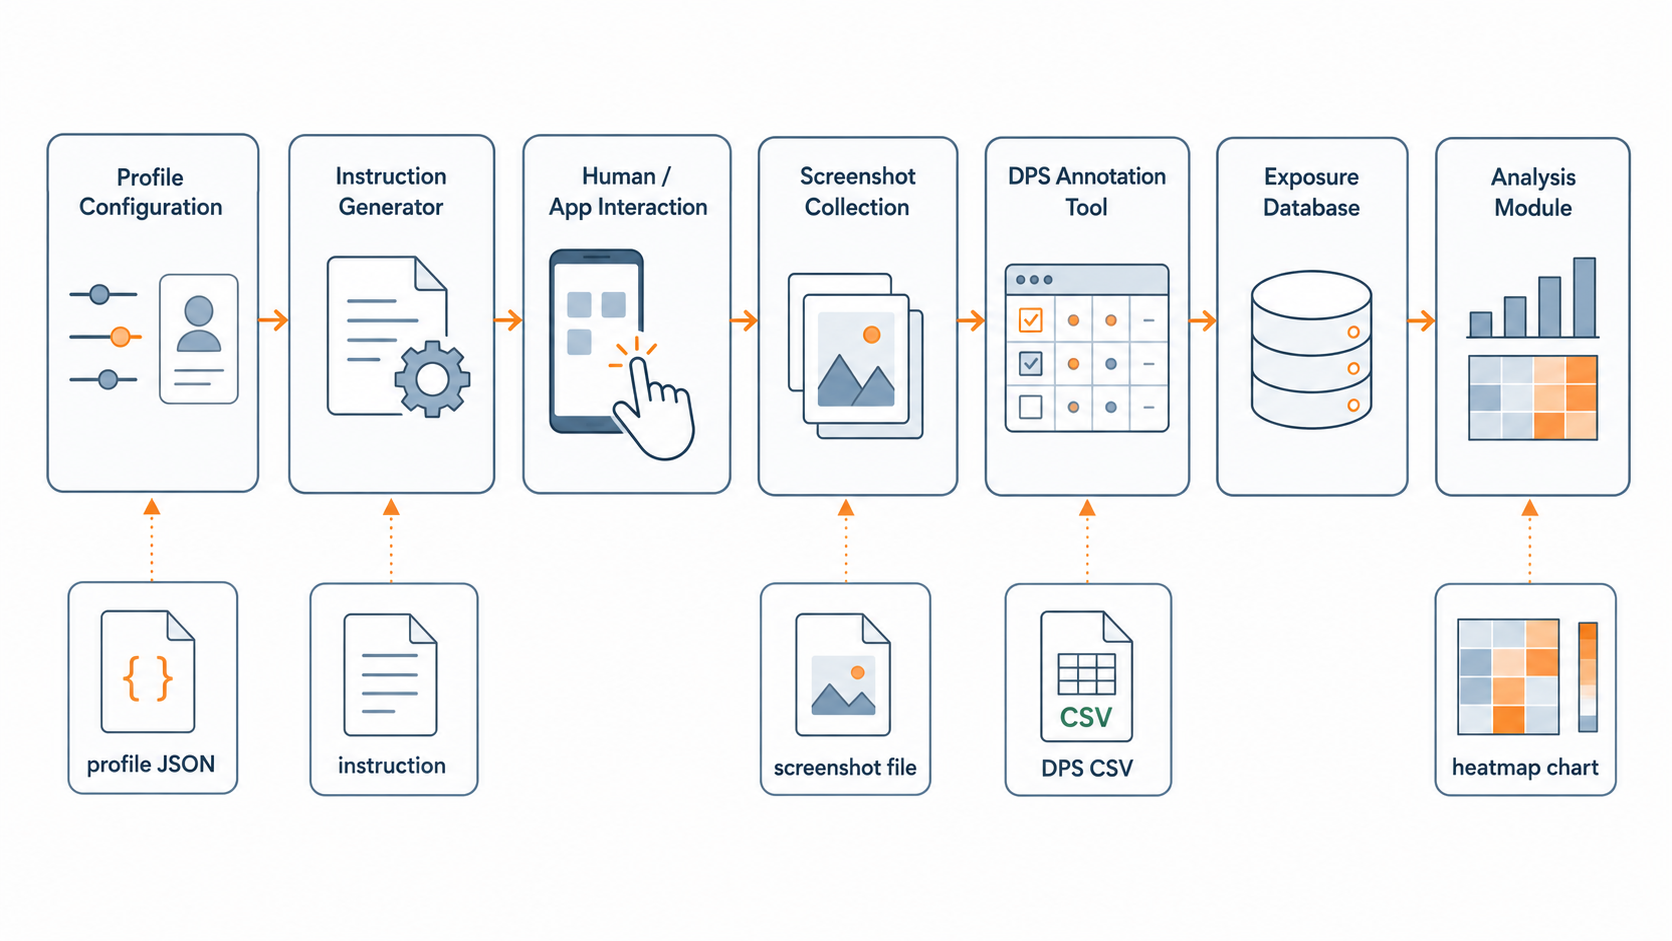
\includegraphics[width=0.95\linewidth]{figures/pictures/system_architecture.png}
    \caption{System Architecture}
    \label{fig:system-architecture}
\end{figure}

\section{Auditing Pipeline Overview}

The system is designed as a profile-aware auditing pipeline that converts abstract user profiles into concrete app interaction trajectories and then into measurable dark-pattern exposure data. Rather than treating dark patterns as static interface elements that can be observed from a single screen, the framework records how exposure emerges during repeated interactions under controlled user assumptions. This design follows the broader logic of black-box auditing, where the internal mechanisms of a platform are not directly accessible, but their observable outputs can be compared under controlled experimental conditions \cite{sandvig2014auditing,srba2023youtube,haroon2023youtubeaudit}.

The pipeline begins with Profile Configuration, where each user profile is defined through behavior probabilities and interest-related keyword distributions. At the beginning of each app-profile run, the workbench loads the configuration, fixes the pseudo-random seed, creates a timestamped run directory, and initializes an empty step record. The system then performs Action Sampling based on the behavior distribution of the selected profile. If the sampled action is search-oriented, the keyword category and concrete keyword are sampled from the profile-specific keyword distribution. The sampled action and keyword are passed to the Instruction Generation module, which translates them into a concrete natural-language interaction instruction. A human operator or semi-automated executor then performs the corresponding App Interaction on a mobile application. After the interaction, the system waits for a fixed delay and collects a Screenshot using a consistent naming and storage convention. The screenshot is then reviewed in the DPS Annotation Tool, where annotators assign seven DPS dimensions: Interface Interference, Friction, Pressure, Contextual Deception, Sneaking, Nagging, and Forced Action. Finally, the annotated step is appended to the Exposure Database and used by the Analysis Module to estimate profile-conditioned exposure and differential exposure patterns.

The complete pipeline can be summarized as:
\[
\text{Profile Configuration} \rightarrow \text{Run Initialization} \rightarrow \text{Action/Keyword Sampling} \rightarrow \text{Instruction Generation} \rightarrow \text{App Interaction} \rightarrow \text{Screenshot Collection} \rightarrow \text{DPS Annotation} \rightarrow \text{Step Persistence} \rightarrow \text{Differential Analysis}.
\]
This implementation structure ensures that the experiment is not merely a collection of screenshots, but a controlled transformation from profile assumptions to interaction traces and then to structured exposure measurements. In the project scale, the framework supports 16 applications, 3 profiles, and 30 interaction steps per profile-app pair, producing 1,440 interaction records and 10,080 DPS labels.

One practical feature of the workflow is that persistence happens after every annotated step rather than only after a full run is completed. The workbench writes both \texttt{steps.jsonl} and \texttt{steps.csv} in the current run directory after each valid step, so interrupted annotation sessions do not invalidate previously collected evidence. The operator can also stop a run early or undo the most recent step before continuing. These controls make the workflow closer to an auditable experiment log than a one-time screenshot collection process.

\section{Repository Structure}
\label{subsec:repository-structure}

The implementation is organized so that profile definitions, generated interaction records, screenshots, analysis scripts, and figures can be traced from the repository rather than from informal experiment notes. The main repository components are:

\begin{itemize}
	\item \texttt{codes/config.json}: profile-independent experiment configuration, including the maximum number of steps, screenshot delay, output directory, and random seed.
	\item \texttt{codes/profiles.json}: profile configuration file containing controlled profile definitions, behavior distributions, keyword pools, and keyword probabilities.
	\item \texttt{codes/main.py}: instruction generator and interactive audit workbench. It samples actions and keywords, generates executable instructions, records screenshots when automatic screenshot support is available, collects DPS annotations, supports undo and early-stop operations, and writes step-level records.
	\item \texttt{results/\{app\}/\{profile\}/\{run\_id\}/screenshots/}: screenshot folder for each app-profile run. Screenshots are stored at the step level and are linked from the corresponding record.
	\item \texttt{results/\{app\}/\{profile\}/\{run\_id\}/steps.csv} and \texttt{steps.jsonl}: annotation files containing the sampled action, keyword category, keyword, generated instruction, screenshot path, DPS scores, timestamp, and optional notes for each interaction step.
	\item \texttt{codes/scripts/analysis\_curve.py}, \texttt{codes/scripts/analysis\_heatmap.py}, and \texttt{codes/scripts/statistical\_tests.py}: analysis scripts used to compute running means, exposure heatmaps, and statistical validation outputs.
	\item \texttt{figures/} and \texttt{figures/statistics/}: figure output folders containing heatmaps, convergence curves, and statistical-test visualizations used in the report.
\end{itemize}

This structure separates configuration, execution, annotation, and analysis. A repeated audit can therefore reuse the same profile configuration and random seed, inspect the generated instructions and screenshots, and regenerate the analysis outputs from the saved step-level annotation files.

\section{Profile Configuration Module}

The profile configuration module defines the experimental conditions under which each audit trajectory is generated. Each profile is stored as a structured configuration rather than as an informal description. This module records the profile name, the behavior probability distribution, the keyword pools, the keyword probabilities, the app category, and the interaction budget. In this project, the three controlled profiles are the high-payment shopping profile, the low-payment browsing profile, and the bargain-hunter profile.

The behavior probability distribution specifies how frequently a profile is expected to perform different interaction actions, such as browsing, searching, visiting a decision-related interface, or returning to a previous page. The keyword pool defines the interest vocabulary available to the profile, while the keyword probabilities determine how likely each keyword is to be selected during search-oriented actions. For example, a high-payment shopping profile may be more associated with high-value electronics or premium product-related keywords, while a bargain-hunter profile may be more associated with discount, coupon, group-buy, or flash-sale terms. These probabilities are not intended to fully model real users. Instead, they create controlled and reproducible approximations of different interest-behavior patterns.

This configuration-based design is important for reproducibility. Since the same profile configuration can be reused across applications and repeated experimental runs, the framework reduces ambiguity in how profiles are operationalized. It also makes profile differences explicit: if two profiles receive different DPS exposure patterns, the comparison can be traced back to controlled differences in their behavior and keyword distributions rather than to undefined user characteristics. Consistent with the ethical scope of the project, demographic attributes are excluded from the configuration. The system therefore audits profile-conditioned exposure through interests and behaviors, not through sensitive personal identities.

In the operational layer, the system may use a finer-grained action vocabulary than the four conceptual categories defined in Chapter~\ref{sec:conceptual-framework}. For example, concrete action tokens can include:

\begin{itemize}
    \item \texttt{visit\_homepage}
    \item \texttt{search\_keyword}
    \item \texttt{browse\_or\_scroll\_page}
    \item \texttt{click\_recommended\_item}
    \item \texttt{like\_or\_favorite}
    \item \texttt{follow\_account}
    \item \texttt{stay\_on\_content}
    \item \texttt{decision\_interface\_visit}
    \item \texttt{close\_popup}
    \item \texttt{back}
\end{itemize}

Before the records are analyzed, these operational actions are mapped back to home, search, browse, and decision so that the behavioral distributions remain comparable at the conceptual level.

\section{Instruction Generation Module}

The instruction generation module serves as the bridge between probabilistic profile configuration and concrete mobile interaction. For each step, the module samples an action from the behavior distribution of the active profile. If the sampled action is a search action, the module further samples a keyword from the profile-specific keyword pool according to the keyword probabilities. The sampled action and keyword are then converted into a natural-language instruction that can be followed during app interaction.

For example, when the sampled action is a keyword search, the generated instruction may be:
\[
\text{`Enter the keyword \{keyword\} in the search box, click the first natural or recommended result, wait for three seconds, and take a screenshot.''}
\]
When the sampled action is browsing or scrolling, the instruction may be:
\[
\text{`Scroll the current page, stop at the first visible promotional or decision-related interface, wait for three seconds, and take a screenshot.''}
\]
These instructions are intentionally concrete. They specify what to do, what kind of interface to stop at, how long to wait, and when to collect evidence. This reduces arbitrary decision-making during interaction and makes the audit procedure easier to repeat.

The current workbench keeps the executor in the loop rather than fully automating app control. The program samples the action, records the instruction, manages screenshots and annotations, and persists the data, while the operator performs the mobile interaction according to the displayed instruction. This implementation boundary avoids relying on brittle app-specific automation scripts and makes the same workflow usable across applications with different layouts. To reduce operator discretion, the instruction text is saved with each step record, so later inspection can verify what the operator was asked to do before the screenshot was captured.

The module does not attempt to infer the internal logic of the application. It only generates external interaction prompts based on controlled profile assumptions. In this sense, the instruction generation module operationalizes profile-conditioned behavior without claiming to simulate the full complexity of real user activity. It provides a practical compromise between experimental control and ecological relevance: the actions are simple enough to standardize, but still close to common app behaviors such as searching, browsing, clicking recommended content, and entering decision-related interfaces.

\section{Screenshot Collection}

Screenshot collection provides the visual evidence for subsequent DPS annotation. After each generated instruction is executed, the framework requires a fixed waiting time before capturing the screen. In this project, the instruction examples use a three-second waiting period. This short delay allows the interface to finish loading dynamic content, recommendation results, pop-ups, or promotional elements before the screenshot is recorded. Although network and device conditions can still introduce variation, using a fixed waiting time improves consistency across steps.

The system also uses a consistent naming convention for screenshots:
\[
\texttt{results/\{app\_name\}/\{profile\_name\}/\{run\_id\}/screenshots/step\_\{step\_id\}.png}
\]
This format encodes the application, profile, run identifier, and step number directly in the file path. It makes screenshots easier to trace, inspect, and match with database records. The run identifier is important because the same app-profile condition may be repeated; without it, repeated runs could overwrite or mix screenshots from different sessions. For example, the screenshot for the seventh step of a high-payment shopping profile in a given app would be stored under that app, profile, and timestamped run directory with the file name \texttt{step\_007.png}.

The implementation supports both automatic and manual screenshot collection. If screenshot automation is available through the local environment, the workbench captures the screen after the configured delay. If automatic capture is unavailable, the workbench prints the expected file path and allows the operator to place a manually captured screenshot there before continuing. This fallback keeps the workflow usable across operating systems and emulator setups while preserving the same path convention in the saved records.

Device and environment consistency are also important. When possible, the same device configuration, account initialization strategy, screen size, network condition, and app version should be maintained across profiles. In the project, controlled conditions include new accounts, cleared histories, comparable app configurations, and profile-specific changes mainly through keyword pools and action distributions. Privacy protection is also necessary during screenshot collection. Screenshots should avoid exposing personal accounts, private messages, payment credentials, precise locations, or other sensitive information. If such information appears, it should be removed, masked, or excluded from the dataset before analysis.

\section{DPS Annotation Tool}

The DPS annotation tool converts visual observations from screenshots into structured dark-pattern exposure labels. For each screenshot, the tool allows annotators to input the seven DPS dimensions: Interface Interference, Friction, Pressure, Contextual Deception, Sneaking, Nagging, and Forced Action. The implementation records numeric scores rather than only binary labels. In particular, Interface Interference can be coded as an ordinal score, Friction can be coded as the extra operation count required to refuse or exit relative to accepting or continuing, and Nagging can be coded as a repeated-interruption count. Pressure, Contextual Deception, Sneaking, and Forced Action are typically coded as binary indicators. When an analysis requires exposure rates, the raw numeric scores can be converted to binary occurrence indicators by applying \(D_i>0\). When an analysis requires intensity, the raw mean score can be used directly.

The tool also supports correction during annotation. Annotators may undo or revise a previous input if they notice an error, and intermediate records can be saved to avoid data loss during long annotation sessions. This is important because the full experiment produces 1,440 interaction records and 10,080 DPS labels. Without intermediate saving and correction support, the annotation process would be more vulnerable to accidental omissions or inconsistent record keeping.

The annotation interface functions as a measurement layer between raw screenshots and statistical analysis. A screenshot alone is not yet an analyzable exposure record. It must first be interpreted according to the DPS framework and converted into structured labels or scores. For example, a pop-up that visually emphasizes a paid option may be annotated as Interface Interference; a countdown or scarcity message may be annotated as Pressure; a screen that requires login or agreement before continuing may be annotated as Forced Action. The tool therefore standardizes how visual interface evidence becomes data for profile-conditioned exposure estimation while still preserving enough score detail for later robustness checks.

\section{Exposure Database}

The exposure database stores the complete interaction and annotation record for the audit. Each row corresponds to one interaction step under a specific app-profile condition. The database is designed to preserve both the experimental context and the annotated outcome, so that each DPS label can be traced back to its application, profile, action, keyword, screenshot, and annotation notes.

Table~\ref{tab:exposure_database_schema} shows the analysis-ready data schema used by the framework. The current raw output files use closely related implementation names such as \texttt{app}, \texttt{profile\_id}, \texttt{step}, and \texttt{note}; these correspond to \texttt{app\_name}, \texttt{profile}, \texttt{step\_id}, and \texttt{notes} in the normalized schema below. The \texttt{app\_category} field is derived from the repository's app-category mapping used for category-level analysis.

	\begin{table}[htbp]
	\centering
	\caption{Exposure database schema.}
	\label{tab:exposure_database_schema}
	\begin{tabular}{ll}
	\hline
	\textbf{Field} & \textbf{Description} \\
	\hline
	\texttt{app\_name} & Name of the audited mobile application \\
	\texttt{app\_category} & Category of the application, such as shopping or food delivery \\
	\texttt{profile} & Controlled profile used in the interaction step \\
	\texttt{step\_id} & Step number within the profile-app trajectory \\
	\texttt{action} & Action sampled from the profile behavior distribution \\
	\texttt{category} & Keyword category sampled for search-oriented actions \\
	\texttt{keyword} & Sampled keyword if the action involves search \\
	\texttt{instruction} & Natural-language instruction shown to the operator \\
	\texttt{screenshot\_path} & File path of the collected screenshot \\
	\texttt{I} & Interface Interference score \\
	\texttt{F} & Friction score or operation-count difference \\
	\texttt{P} & Pressure score or indicator \\
	\texttt{C} & Contextual Deception score or indicator \\
	\texttt{S} & Sneaking score or indicator \\
	\texttt{N} & Nagging score or interruption count \\
	\texttt{FA} & Forced Action score or indicator \\
	\texttt{timestamp} & Time at which the record was created or annotated \\
	\texttt{notes} & Optional comments for ambiguous or notable cases \\
	\hline
	\end{tabular}
	\end{table}

This schema supports both traceability and aggregation. At the lowest level, researchers can inspect a single screenshot and its labels. At a higher level, the same records can be grouped by profile, app, app category, action type, or DPS dimension. The database therefore acts as the central connection between implementation and analysis.

\section{Analysis Module}

The analysis module computes exposure estimates and differential exposure statistics from the exposure database. At the profile level, it estimates profile-conditioned exposure \(E(D \mid A)\), where \(A\) denotes a controlled profile and \(D\) denotes a DPS dimension or DPS vector. Depending on the analysis mode, \(D\) can refer either to the raw DPS score or to a binary occurrence variable \(1[D_i>0]\). The former summarizes exposure intensity, while the latter summarizes how frequently a profile encounters each type of dark-pattern exposure across its interaction trajectory. At the app level, the module aggregates DPS labels within each application. At the category level, it further groups applications into broader categories, allowing the project to examine whether certain app categories are associated with consistently higher exposure in specific DPS dimensions.

The module also computes pairwise exposure differences:
\[
\Delta(A_i, A_j) = E(D \mid A_i) - E(D \mid A_j).
\]
This comparison is used to examine whether two controlled profiles receive different dark-pattern exposure patterns under comparable experimental conditions. The framework does not interpret such differences as direct causal proof of personalization. Instead, it treats them as observable profile-conditioned exposure gaps that may be associated with differences in behavior distributions, keyword interests, app responses, or decision-interface triggers.

Several visualization and statistical components are included. Heatmaps display exposure patterns across profiles, applications, categories, and DPS dimensions. Running mean convergence curves track how exposure estimates change as interaction steps accumulate, helping assess whether the estimates gradually stabilize over repeated interactions. The representative heatmaps and statistical validation plots are reported in Chapter~\ref{chap:results}, with the full visualization set collected in Appendix~\ref{app:full-heatmaps}.

For statistical validation, the analysis module supports permutation tests, q-values for multiple-testing correction, L1 distance, Cramér’s V, Welch's \(t\)-tests, and Mann--Whitney \(U\) tests. Permutation tests compare observed profile gaps against gaps obtained under randomized profile assignments. Q-values reduce the risk of overinterpreting repeated significance tests across multiple DPS dimensions or app categories. L1 distance measures the magnitude of difference between DPS exposure vectors, while Cramér’s V provides an association measure between profile type and exposure labels. The chi-square contingency analysis can be run in binary mode, where each nonzero DPS score counts as one occurrence, or in score mode, where raw DPS scores are summed. Together, these outputs allow the report to discuss both statistical evidence and practical exposure differences without relying on a single metric.
